%% Template originaly created by Karol Kozioł (mail@karol-koziol.net) and modified for ShareLaTeX use

\documentclass[a4paper,13pt]{article}
\usepackage[linesnumbered,algoruled,boxed,lined]{algorithm2e}
\usepackage{multirow}
\usepackage[T1]{fontenc}
\usepackage[utf8]{inputenc}
\usepackage{graphicx}
\usepackage{xcolor}
\renewcommand\familydefault{\rmdefault}
\usepackage{tgheros}

\usepackage{amsmath,amssymb,amsthm,textcomp}
\usepackage{enumerate}
\usepackage{multicol}
\usepackage{tikz}
\usepackage[utf8]{vietnam}
\usepackage[unicode]{hyperref}
\usepackage{mathtools}
\usepackage[]{mdframed}

% draw a frame around given text
\newcommand{\framedtext}[1]{%
\par%
\noindent\fbox{%
    \parbox{\dimexpr\linewidth-2\fboxsep-2\fboxrule}{#1}%
}%
}
\newcommand\Myperm[2][^n]{\prescript{#1\mkern-2.5mu}{}P_{#2}}
\newcommand\Mycomb[2][^n]{\prescript{#1\mkern-0.5mu}{}C_{#2}}
\usepackage{geometry}
\geometry{total={210mm,297mm},
left=25mm,right=25mm,%
bindingoffset=0mm, top=22mm,bottom=25mm}

\linespread{1.3}

\newcommand{\linia}{\rule{\linewidth}{0.5pt}}

% custom theorems if needed
\newtheoremstyle{mytheor}
    {1ex}{1ex}{\normalfont}{0pt}{\scshape}{.}{1ex}
    {{\thmname{#1 }}{\thmnumber{#2}}{\thmnote{ (#3)}}}

\theoremstyle{mytheor}
\newtheorem{defi}{Definition}

% my own titles
\makeatletter
\renewcommand{\maketitle}{
\begin{center}
\vspace{2ex}
{\huge \textsc{\@title}}
\vspace{1ex}
\\
\linia\\
\@author \hfill \@date
\vspace{4ex}
\end{center}
}
\makeatother
%%%

% custom footers and headers
\usepackage{fancyhdr}
\setlength{\headheight}{20pt}
\pagestyle{fancy}
\fancyhead{} % clear all header fields
\fancyhead[L]{
 \begin{tabular}{rl}
    \begin{picture}(15,10)(0,0)
    \put(0,-8){
\includegraphics[width=8mm, height=8mm]{hcmut.png}}
    %\put(0,-8){\epsfig{width=10mm,figure=hcmut.eps}}
   \end{picture}&
	%
\includegraphics[width=8mm, height=8mm]{hcmut.png} & %
	\begin{tabular}{l}
		\textbf{\bf \ttfamily Ho Chi Minh City, University of Technology}\\
		\textbf{\bf \ttfamily Department of Computer Science and Engineer}
	\end{tabular} 	
 \end{tabular}
}
\fancyhead[R]{
	\begin{tabular}{l}
		\tiny \bf \\
		\tiny \bf 
	\end{tabular}  }
\fancyfoot{} % clear all footer fields
\fancyfoot[L]{\scriptsize \ttfamily Nghiên cứu phát triển kỹ thuật đếm số phần tử trên dòng dữ liệu}
\rfoot{Trang \thepage}
\renewcommand{\headrulewidth}{0.2pt}
\renewcommand{\footrulewidth}{0.2pt}
%

\usepackage{xcolor}
\definecolor{block-gray}{gray}{0.85}

\usepackage{environ}

\NewEnviron{myblock}
{
    \colorbox{block-gray}
    {
        \parbox{\dimexpr\linewidth-2\fboxsep\relax}
        {
            \bigbreak
            \addtolength{\leftskip}{4mm}
            \addtolength{\rightskip}{4mm}
            \BODY
        }
    }
}
\renewcommand{\quote}{\myblock}
\renewcommand{\endquote}{\endmyblock}
% code listing settings
\usepackage{listings}
\lstset{
    language=Python,
    basicstyle=\ttfamily\small,
    aboveskip={1.0\baselineskip},
    belowskip={1.0\baselineskip},
    columns=fixed,
    extendedchars=true,
    breaklines=true,
    tabsize=4,
    prebreak=\raisebox{0ex}[0ex][0ex]{\ensuremath{\hookleftarrow}},
    frame=lines,
    showtabs=false,
    showspaces=false,
    showstringspaces=false,
    keywordstyle=\color[rgb]{0.627,0.126,0.941},
    commentstyle=\color[rgb]{0.133,0.545,0.133},
    stringstyle=\color[rgb]{01,0,0},
    numbers=left,
    numberstyle=\small,
    stepnumber=1,
    numbersep=10pt,
    captionpos=t,
    escapeinside={\%*}{*)}
}
%%%----------%%%----------%%%----------%%%----------%%%

\begin{document}

\begin{titlepage}
\begin{center} {\textbf{ĐẠI HỌC QUỐC GIA TP. HỒ CHÍ MINH}
}

{\textbf{TRƯỜNG ĐẠI HỌC BÁCH KHOA}
}

{\textbf{KHOA KHOA HỌC VÀ KỸ THUẬT MÁY TÍNH }
}

{\textbf{---------------------------------------}}

\end{center}

\vspace{1cm}

\begin{figure}[h!]
\begin{center}

\includegraphics[width=3cm]{hcmut.png}
\end{center}
\end{figure}

\vspace{2cm}


\begin{center}
\begin{tabular}{c}
\multicolumn{1}{c}{\textbf{\Large NGHIÊN CỨU PHÁT TRIỂN KỸ THUẬT ĐẾM SỐ PHẦN TỬ TRÊN DÒNG DỮ LIỆU}}
\vspace{2cm}
\\
\multicolumn{1}{c}{\textbf{\Large LUẬN VĂN THẠC SĨ}}


~~\\

\\
\multicolumn{1}{l}{\textbf{{\Large}}}\\
\\
\textbf{{\Large}}\\

\\
\\

\end{tabular}
\end{center}

\vspace{1cm}

\begin{table}[h]
\begin{tabular}{rrl}
\hspace{5.1cm} 
&\textit{Học viên: } & \textbf{LÊ ANH QUỐC}\\
&\textit{ID: } & \textbf{2070428}\\

\end{tabular}
\end{table}
\vspace{3cm}
\begin{center}
{\footnotesize HỒ CHÍ MINH CITY}
\end{center}
\end{titlepage}

\begin{titlepage}
\begin{center} {\textbf{ĐẠI HỌC QUỐC GIA TP. HỒ CHÍ MINH}
}

{\textbf{TRƯỜNG ĐẠI HỌC BÁCH KHOA}
}

{\textbf{KHOA KHOA HỌC VÀ KỸ THUẬT MÁY TÍNH }
}

{\textbf{---------------------------------------}}

\end{center}

\vspace{1cm}

\begin{figure}[h!]
\begin{center}

\includegraphics[width=3cm]{hcmut.png}
\end{center}
\end{figure}

\vspace{2cm}


\begin{center}
\begin{tabular}{c}
\multicolumn{1}{c}{\textbf{\Large NGHIÊN CỨU PHÁT TRIỂN KỸ THUẬT ĐẾM SỐ PHẦN TỬ TRÊN DÒNG DỮ LIỆU}}
\vspace{2cm}
\\
\multicolumn{1}{c}{\textbf{\Large LUẬN VĂN THẠC SĨ}}

\vspace{0.5cm}
\\
\multicolumn{1}{c}{\text{\small NGÀNH: KHOA HỌC MÁY TÍNH }}
\vspace{0.5cm}
\\
\multicolumn{1}{c}{\text{\small MÃ NGÀNH: \textbf{8480101} }}
\vspace{1cm}
\\
\multicolumn{1}{c}{\textbf{\small NGƯỜI HƯỚNG DẪN KHOA HỌC }}
~~\\
\multicolumn{1}{c}{\textbf{\small PGS. TS. THOẠI NAM
 }}

\\
\\

\\
\\

\end{tabular}
\end{center}

\vspace{1cm}

\begin{table}[h]
\begin{tabular}{rrl}
\hspace{5.6cm} 
&\textit{Học viên: } & \textbf{lÊ ANH QUỐC}\\
&\textit{ID: } & \textbf{2070428}\\

\end{tabular}
\end{table}
\vspace{1cm}
\begin{center}
{\footnotesize HỒ CHÍ MINH CITY}
\end{center}
\end{titlepage}

%%%----------%%%----------%%%----------%%%----------%%%


%\thispagestyle{empty}

\renewcommand{\contentsname}{Content}
\newpage
\vspace{1cm}
\tableofcontents
\newpage
\section{GIỚI THIỆU ĐỀ TÀI, MỤC TIÊU VÀ ĐỐI TƯỢNG NGHIÊN CỨU}
\subsection{Tính cấp thiết và lý do chọn đề tài}
\hspace{2em}Ngày nay, các ứng dụng và dịch vụ trực tuyến đóng vai trò ngày càng quan trọng trong cuộc sống của con người. 
Chúng ta sử dụng mạng xã hội để kết nối với bạn bè và chia sẻ thông tin, mua sắm trực tuyến để tiết kiệm thời gian và tiền bạc, 
hay xem phim và chơi game trực tuyến để giải trí. Để đánh giá hiệu quả hoạt động của các ứng dụng và dịch vụ này, 
một trọng những chỉ số quan trọng nhất là số lượng người dùng hoạt động.

Việc theo dõi số lượng người dùng hoạt động trong một khoảng thời gian nhất định trên một dòng dữ liệu (data stream) 
là một yêu cầu quan trọng đối với nhiều ứng dụng và dịch vụ trực tuyến, hiệu quả của các chiến dịch marketing, 
và hỗ trợ ra quyết định kinh doanh.\\
Ví dụ, trong các ứng dụng mạng xã hội, số lượng người dùng hoạt động cho thấy mức độ tương tác 
và sự quan tâm của người dùng đối với nền tảng. Trong các dịch vụ thương mại điện tử, số lượng người dùng hoạt động cho thấy hiệu quả 
và các chiến dịch quảng cáo và khuyến mãi. \\
Tuy nhiên, việc đếm số lượng người dùng không phải là một nhiệm vụ đơn giản, đặc biệt là khi dữ liệu lớn 
và tốc độ truy cập cao. Các phương pháp truyền thống như lưu trữ và truy vấn trực tiếp vào cơ sở dữ liệu có thể gặp nhiều hạn chế về hiệu suất 
và khả năng mở rộng.\\

Trong nhiều trường hợp, cần phải tổng hợp số lượng người dùng trên nhiều dòng dữ liệu khác nhau. Việc này giúp có được bức tranh toàn cảnh về hoạt động 
của người dùng trên toàn hệ thống, từ đó đưa ra các phân tích và đánh giá chính xác hơn.\\
Ví dụ, trong hệ thống thương mại điện tử, cần tổng hợp số lượng người dùng từ các trang web, ứng dụng di động và API khác nhau để có được số lượng 
người dùng hoạt động thực tế trên toàn hệ thống. 
Tuy nhiên, việc tổng hợp dữ liệu từ nhiều nguồn khác nhau có thể gặp thách thức về đồng bộ hóa dữ liệu, xử lý dữ liệu bị thiếu hoặc lỗi, 
và đảm bảo tính nhất quán của kết quả. 

Ngoài ra, có thể cần phải đếm số lượng người dùng trên nhiều khoảng thời gian khác nhau trên một hoặc nhiều dòng dữ liệu khác nhau. 
Việc này giúp phân tích chi tiết hơn hoạt động của người dùng theo thời gian, theo khu vực hoặc theo tiêu chí khác.\\
Ví dụ, trong một ứng dụng phát trực tiếp, cần đếm số lượng người dùng hoạt động theo giờ hoặc từng phân đoạn chương trình 
để đánh giá mức độ quan tâm của người xem. Tuy nhiên, việc phân chia và xử lý dữ liệu theo nhiều đoạn có thể làm 
tăng độ phức tạp của thuật toán và ảnh hưởng đến hiệu suất của hệ thống. Do đó, cần phải có một giải pháp 
đếm số lượng phần tử trên dòng dữ liệu đạt hiệu suất cao và tin cậy, từ đó có thể ứng dụng rộng rãi trong các 
hệ thống khác nhau như mạng xã hội, thương mại điện tử, chương trình phát trực tiếp, hệ thống giám sát 
và hệ thống giao thông thông minh.

\section{Mục tiêu nghiên cứu}
\subsubsection{Phát triển thuật toán để ước lượng số lượng phần tử (cardinality estimation) trên một dòng dữ liệu (data stream):}
\subsubsection{Mở rộng thuật toán để ước lượng số lượng phần tử trong một khoảng thời gian trên nhiều streams:}
\subsubsection{Phát triển một thuật toán để ước lượng số lượng phần tử trên nhiều khung thời gian tỏng hợp từ nhiều dòng dữ liệu}

\section{Giới hạn và đối tượng nghiên cứu }
\subsubsection{Giới hạn}
\subsubsection{Đối tượng nghiên cứu }
Đối tượng nghiên cứu của đề tài "Nghiên cứu phát triển kỹ thuật đếm số lượng phần tử trên dòng dữ liệu"

\section{CÁC CÔNG TRÌNH NGHIÊN CỨU LIÊN QUAN }
- \textbf{LogLog} – [1] \\

- \textbf{HyperLogLog} – [2]\\

- \textbf{HyperLogLog++} - [3] \\

- \textbf{Sliding HyperLogLog} - [4]\\

- \textbf{ExaLogLog} - [5] \\

\section{HyperLogLog}
Vấn đề ước lượng số lượng phần tử (\textit{cardinality estimation problem}) là một nhiệm vụ để tìm số lượng phần tử phân biệt 
trong một tập dữ liệu trong đó có sự xuất hiện của các bản sao (duplicates). Truyền thống, 
để xác định số lượng chính xác của một tập hợp, các phương pháp cổ điển xây dựng 
một danh sách của tất cả các phần tử và sử dụng sắp xếp và tìm kiếm để tránh liệt kê 
các phần tử nhiều lần. Đếm số lượng phần tử trong danh sách đó cho phép tính chính xác 
số lượng các phần tử duy nhất, nhưng nó có độ phức tạp thời gian là $O(N\cdot logN)$, 
trong đó N là số lượng tất cả các phần tử bao gồm cả các bản sao, và yêu cầu 
bộ nhớ phụ tuyến tính, điều này không thể thực hiện được đối với các ứng dụng 
Big Data với tập dữ liệu lớn có độ phức tạp lớn.
\begin{mdframed}
   \textbf{Ví dụ 3.1: Số lượng khách truy cập}\\
    Một trong những chỉ số KPI quý giá cho bất kỳ trang web nào là số lượng khách truy cập duy nhất đã ghé thăm trong một khoảng thời gian cụ thể. 
    Để đơn giản, chúng ta giả định rằng khách truy cập duy nhất sử dụng các địa chỉ IP khác nhau, do đó chúng ta cần tính toán số lượng địa chỉ IP 
    duy nhất mà theo giao thức Internet IPv6 được biểu diễn bằng chuỗi 128-bit. Liệu đây có phải là một nhiệm vụ dễ dàng không? 
    Chúng ta có thể chỉ sử dụng các phương pháp cổ điển để đếm số lượng một cách chính xác không? Điều này phụ thuộc vào sự phổ biến của trang web.\\
    Xem xét thống kê lưu lượng cho tháng 3 năm 2017 của ba trang web bán lẻ phổ biến nhất tại Hoa Kỳ: \textit{amazon.dot, ebay.com} và 
    \textit{walmart.com}. Theo SimilarWeb, số lần truy cập trung bình đến các trang web đó là khoảng 1,44 tỷ và số lượng trang xem trung bình 
    mỗi lần truy cập là 8,24. Do đó, thống kê cho tháng 3 năm 2017 bao gồm khoảng 12 tỷ địa chỉ IP với mỗi địa chỉ có 128-bit, tức là tổng 
    kích thước là 192 GB.\\
    Nếu chúng ta giả định rằng mỗi 10 người trong số những khách truy cập đó là duy nhất, chúng ta có thể mong đợi số lượng phần tử 
    trong tập hợp đó là khoảng 144 triệu và bộ nhớ cần thiết để lưu trữ danh sách các phần tử duy nhất là 23 GB.
\end{mdframed}
\break
Một ví dụ khác minh họa thách thức của việc ước lượng số lượng phần tử 
cho các nhà nghiên cứu khoa học.
\begin{mdframed}
    \textbf{Example 3.2: DNA analysis (Giroire, 2016)}\\
    Một trong những nhiệm vụ lâu dài trong nghiên cứu gen con người là nghiên cứu sự tương quan trong các chuỗi DNA. Các phân tử DNA 
    bao gồm hai chuỗi kết hợp, mỗi chuỗi được tạo thành từ bốn đơn vị cơ bản của DNA, được đánh dấu là A (adenine), G (guanine), C (cytosine), và T (thymine). Gen con người chứa khoảng 3 tỷ cặp cơ sở DNA như vậy. Việc xác định chuỗi DNA có nghĩa là xác định thứ tự chính xác của các cặp cơ sở trong một đoạn DNA.\
    Từ quan điểm toán học, một chuỗi DNA có thể được coi là một chuỗi các biểu tượng A, G, C, T có thể dài bất kỳ, và chúng ta có thể coi chúng như 
    một ví dụ của một tập dữ liệu có thể vô hạn.\\
    Vấn đề đo lường tương quan có thể được sử dụng làm một nhiệm vụ xác định số lượng các chuỗi con phân biệt có kích thước cố định trong một phần của DNA. 
    Ý tưởng là một chuỗi với một số lượng chuỗi con phân biệt ít hơn sẽ có sự tương quan cao hơn so với một chuỗi cùng kích thước nhưng có nhiều chuỗi con 
    phân biệt hơn.\\
    Các thí nghiệm như vậy đòi hỏi nhiều lần chạy trên nhiều tập tin lớn và để tăng tốc cho nghiên cứu, họ yêu cầu chỉ có bộ nhớ giới hạn hoặc thậm chí 
    là bộ nhớ không đổi và thời gian thực thi nhỏ, điều này không thể thực hiện được với các thuật toán đếm chính xác.
\end{mdframed}
Do đó, những lợi ích có thể đạt được từ việc ước lượng số lượng phần tử chính xác được bỏ qua do yêu cầu xử lý thời gian lớn và bộ nhớ lớn. 
Các ứng dụng Big Data sẽ sử dụng các phương pháp thực tế hơn, chủ yếu dựa trên các thuật toán xác suất khác nhau, ngay cả khi chúng chỉ cung cấp 
các câu trả lời xấp xỉ.\\
\vspace{0.5cm}
\begin{quote}
    Trong quá trình xử lý dữ liệu, việc hiểu về kích thước của tập dữ liệu và số lượng các phần tử phân biệt có thể xuất hiện là rất quan trọng.\\
    Hãy xem xét chuỗi tiềm năng vô hạn các ký tự đơn a, d, s, ..., dựa trên các chữ cái từ bảng chữ cái tiếng Anh. 
    Số lượng các phần tử có thể ước lượng dễ dàng và nó được chặn trên bởi số lượng chữ cái, là 26 trong ngôn ngữ tiếng Anh hiện đại. 
    Rõ ràng, trong trường hợp này, không cần áp dụng bất kỳ phương pháp xác suất nào và một giải pháp đơn giản dựa trên từ điển để tính toán chính xác 
    số lượng phần tử hoạt động rất tốt.\\
\end{quote}
\indent Để tiếp cận vấn đề về số lượng phần tử, nhiều trong số các phương pháp xác suất phổ biến được ảnh hưởng bởi các ý tưởng của thuật toán Bloom filter, 
chúng hoạt động trên các giá trị băm của các phần tử, sau đó quan sát các mẫu phân phối phổ biến và đưa ra các \textquotedblleft\textit{phỏng đoán}\textquotedblright có lý về số lượng 
phần tử duy nhất mà không cần phải lưu trữ tất cả chúng.
\subsection{Linear Counting}
\indent Như một phương pháp xác suất đầu tiên cho vấn đề về số lượng phần tử, chúng ta xem xét thuật toán đếm xác suất có thời gian tuyến tính, 
gọi là thuật toán \textit{Linear Counting}. Các ý tưởng gốc của thuật toán này đã được đề xuất bởi Morton Astrahan, Mario Schkolnick và Kyu-Young Whang 
vào năm 1987 [As87], và thuật toán thực tế đã được công bố bởi Kyu-Young Whang, Brad Vander-Zanden và Howard Taylor vào năm 1990 [Wh90].\\
Cải tiến ngay lập tức đối với các phương pháp chính xác cổ điển là băm các phần tử bằng một hàm băm \textit{h}, mà có thể loại bỏ các bản sao mà 
không cần sắp xếp các phần tử với chi phí của việc giới thiệu một số lượng xác suất sai sót do các va chạm băm có thể 
xảy ra (chúng ta không thể phân biệt giữa các bản sao và "bản sao ngẫu nhiên"). Do đó, việc sử dụng một bảng băm như vậy chỉ yêu cầu một 
quy trình quét thích hợp để thực hiện một thuật toán đơn giản mà đã vượt trội hơn phương pháp cổ điển.\\
\indent Tuy nhiên, đối với các tập dữ liệu có số lượng phần tử lớn, các bảng băm như vậy có thể khá lớn và yêu cầu bộ nhớ tăng lên tuyến tính với 
số lượng phần tử phân biệt trong tập hợp. Đối với các hệ thống có bộ nhớ hạn chế, điều này sẽ đòi hỏi bộ nhớ đĩa hoặc lưu trữ phân tán ở một số 
điểm nào đó, điều này giảm đáng kể các lợi ích của bảng băm do truy cập đĩa chậm hoặc mạng.\\
\indent Tương tự như ý tưởng của bộ lọc Bloom, để giải quyết vấn đề này, thuật toán Linear Counting không lưu trữ các giá trị băm chính mà chỉ 
các bit tương ứng của chúng, thay thế bảng băm bằng một mảng bit LINEARCOUNTER có độ dài \textit{m}. Giả sử rằng \textit{m} vẫn tỷ lệ với 
số lượng dự kiến các phần tử phân biệt \textit{n}, nhưng chỉ yêu cầu 1 bit cho mỗi phần tử, điều này khả thi cho hầu hết các trường hợp.\\
\indent Ban đầu, tất cả các bit trong LINEARCOUNTER đều bằng không. Để thêm một phần tử mới \textit{x} vào cấu trúc dữ liệu như vậy, 
chúng ta tính toán giá trị băm của nó là \textit{h(x)} và đặt bit tương ứng thành một trong bộ đếm.\\\\
\vspace{0.5cm}
\begin{algorithm}[H]
    \DontPrintSemicolon
    \LinesNumberedHidden
    \caption[]{Adding element to the Linear counter}
    \KwIn{Element $x \in D$}
    \KwIn{Linear counter with hash function $h$}
    $j \gets h(x)$\;
    \If{$LINEARCOUNTER[j] == 5$}
    {
        $LINEARCOUNTER[j]\gets 1$
    }
\end{algorithm}
\indent Vì chỉ sử dụng một hàm băm \textit{h}, chúng ta có thể dự kiến rất nhiều va chạm cứng bổ sung khi hai giá trị băm khác nhau đặt cùng một bit 
trong mảng. Do đó, số lượng chính xác (hoặc gần chính xác) các phần tử phân biệt không thể nữa được trực tiếp lấy từ một bản phác họa như vậy.\\
\indent Ý tưởng của thuật toán dẫn đến việc phân phối các phần tử vào các ngăn (bit được chỉ mục bằng các giá trị băm) và duy trì một mảng 
bit LINEARCOUNTER chỉ ra những ngăn nào bị ảnh hưởng. Quan sát số lần ảnh hưởng trong mảng dẫn đến ước lượng về số lượng phần tử.\\
\indent Trong bước đầu tiên của thuật toán Linear Counting, chúng ta xây dựng cấu trúc dữ liệu LINEARCOUNTER của chúng ta như được hiển thị trong 
Thuật toán 1. Sau khi có bản phác họa như vậy, số lượng có thể được ước tính bằng cách sử dụng tỷ lệ quan sát được của các bit trống \textbf{V} 
theo công thức:\\
\begin{equation}
    n \approx -m\cdot\ln V \tag{$3.1$}
\end{equation}
\indent Bây giờ chúng ta thấy rõ làm thế nào các va chạm ảnh hưởng đến ước lượng về số lượng phần tử trong thuật toán Linear Counting - mỗi đụng độ 
làm giảm số lượng bit phải được đặt, làm cho tỷ lệ quan sát được của các bit chưa được đặt lớn hơn so với giá trị thực tế. Nếu không có đụng độ băm, 
số lượng cuối cùng các bit được đặt sẽ là số lượng phần tử mong muốn. Tuy nhiên, đụng độ là không tránh khỏi và công thức (3.1) thực tế đưa ra một 
ước lượng vượt quá số lượng chính xác và, vì số lượng phần tử là một giá trị số nguyên, chúng ta ưu tiên làm tròn kết quả của nó đến số nguyên nhỏ nhất 
gần nhất.\\
\indent Do đó, chúng ta có thể công thức hóa thuật toán đếm hoàn chỉnh như sau.\\
\vspace{0.5cm}
\begin{algorithm}[H]
    \DontPrintSemicolon
    \LinesNumberedHidden
    \caption[]{Estimating cardinality with Linear Counting}
    \KwIn{Dataset $ D $}
    \KwOut{Cardinality estimation}
    LINEARCOUNTER[j] $\gets 0$, $i = 0$ ... m $- $ 1\;
    \For{x $\in $ D} { LINEARCOUNTER.Add(e) }
    Z $\gets count_{i=1...m-1} (LINEARCOUNTER[i] = 0 $)\;
    \Return{$-m \cdot \ln(\frac{Z}{m})$}
\end{algorithm}
\begin{mdframed}
    \textbf{Example 3.3: Linear Counting algorithm}\\
    Xem xét một tập dữ liệu chứa 20 tên của các thành phố thủ đô được trích xuất từ các bài báo tin tức gần đây: \textbf{Berlin,} Berlin, \textbf{Paris,} Berlin,
    \textbf{Lisbon, Kiev,} Paris, \textbf{London, Rome, Athens, Madrid, Vienna,}
    Rome, Rome, Lisbon, Berlin, Paris, London, Kiev, \textbf{Washington.}\\
    Đối với các số lượng phần tử nhỏ như vậy (số lượng thực sự là 10), để có một sai số tiêu chuẩn khoảng 10\%, chúng ta cần chọn độ dài của 
    cấu trúc dữ liệu LINEARCOUNTER ít nhất bằng số lượng dự kiến của các phần tử duy nhất, do đó hãy chọn $m = 2^4$. Với hàm băm $h$ có giá trị 
    trong ${0,1,...,2^4-1}$, chúng ta sử dụng một hàm dựa trên MurmurHash3 32-bit được định nghĩa như sau:
    \begin{equation}
        h(x) := MurmurHash3(x)\mod m,
      \end{equation}
    và giá trị băm của các thành phố thủ đô có thể được tìm thấy trong bảng dưới đây.
\begin{center}
    \begin{tabular}{ |c|c| }
        \multicolumn{2}{}{} \\ \hline
        \textbf{City} & \textbf{h(City)} \\ \hline
        Athens & 12 \\
        Berlin & 7 \\
        Kiev & 13 \\
        Lisbon & 15 \\
        London & 14 \\
        \cline{1-2}
    \end{tabular}
    \hspace{0.5cm}
    \begin{tabular}{ |c|c| }
        \multicolumn{2}{}{}\\ \hline
        \textbf{City} & \textbf{h(City)} \\ \hline
        Madrid & 14 \\
        Paris & 8 \\
        Rome & 1 \\
        Vienna & 6 \\
        Washington & 11 \\
        \cline{1-2}
    \end{tabular}
\end{center}
Như chúng ta có thể thấy, các thành phố \textbf{London} và \textbf{Madrid} có cùng một giá trị, nhưng các đụng độ như vậy là điều dễ hiểu 
và hoàn toàn tự nhiên. Cấu trúc dữ liệu LINEARCOUNTER có dạng như sau:
\begin{center}
    \begin{tabular}{p{0.4cm}p{0.4cm}p{0.4cm}p{0.4cm}p{0.4cm}p{0.4cm}p{0.4cm}p{0.4cm}p{0.4cm}p{0.4cm}p{0.4cm}p{0.4cm}p{0.4cm}p{0.4cm}p{0.4cm}p{0.4cm}}
        0 & 1 & 2 & 3 & 4 & 5 & 6 & 7 & 8 & 9 & 10 & 11 & 12 & 13 & 14 & 15 % Add bottom border to all rows
    \end{tabular}
    \begin{tabular}{|p{0.4cm}|p{0.4cm}|p{0.4cm}|p{0.4cm}|p{0.4cm}|p{0.4cm}|p{0.4cm}|p{0.4cm}|p{0.4cm}|p{0.4cm}|p{0.4cm}|p{0.4cm}|p{0.4cm}|p{0.4cm}|p{0.4cm}|p{0.4cm}|}
        \hline
        0 & 1 & 0 & 0 & 0 & 0 & 1 & 1 & 1 & 0 & 0 & 1 & 1 & 1 & 1 & 1 \\ \cline{1-16} % Add bottom border to all rows
    \end{tabular}
\end{center}
\vspace{0.2cm}
According to the Linear Counting algorithm, we calculate the fraction \textbf{V}
of empty bits in the LINEARCOUNTER:
\begin{equation}
    V = \frac{9}{16} = 0.5625
\end{equation}
and the estimated cardinality is
\begin{equation}
    n \approx -16\cdot \ln 0.5625 \approx 9.206,
\end{equation}
which is pretty close to th exact number 10.
\end{mdframed}
\subsection*{Properties}
If the hash function $h$ can be computed in a constant time (which is true
for the most popular hash function), the time to process every element is
a fixed constant O(N), where N is the total number of elements, including
duplicates. Thus, the algorithm has O(N) time complexity.\\
\indent As for many other probabilistic algorithm, there is a number of
parameters that can be runed to influence its performance.\\
\indent The expected accuracy of the estimation depends on the bit array
size $m$ and its ratio to the number of distinct elements $\alpha$ = $\frac{m}{n}$, called
the \textit{load factor}. Unless $\alpha$ $\geq$ $1$ ($m$ > $n$ is not practically interesting case),
there is non-zero probability $P_{full}$ that LINEARCOUNTER bit array
becomes full, called the $fill-up probability$, that fatally distorts
the algorithm and blows up the expression (3.1). The probability $P_{full}$
depends on the load factor and, consequently, on the size $m$ that should
be selected big enough to have the fill-up probability negligible.\\
\indent The standard error $\sigma$ is a measure of the variability of the estimate
provided by Linear Counting and there is a trade-off between it and
the bit array zise $m$. Descreasing the standard error results in more
precies estimates, but increase the require memory.\\\\
\begin{quote}
    \begin{center}
        \textbf{Table 3.1:} Trade-off between accuracy and bit array size\\
        \begin{tabular}{|*{3}{c|}}
            \hline
            \multirow{2}{*}{n} & \multicolumn{2}{c|}{\text{m}} \\ \cline{2-3} 
                    & $\sigma = 1\%$ & $\sigma = 10\%$ \\ \hline
            1000 & 5329 & 268 \\ \hline
            10000 & 7960 & 1709 \\ \hline
            100000 & 26729 & 12744 \\ \hline
            10000000 & 154171 & 100880 \\ \hline
            10000000 & 1096582 & 831809 \\ \hline
            100000000 & 8571013 & 7061760 \\ \hline
        \end{tabular}
    \end{center}
\end{quote}\\

The dependence on choosing $m$ is quite complex and has no analysis
solution. However, for a widely acceptable fill-up probabilistic $P_full = 0.7\%$
the algorithm authors have provided precomputed values that are given in Table 3.1
and can be used as references.

Since the fill-up probability is never zero, the bit array very rarely
becomes full and distorts Algorithm 3.2. When working with small
datasets, we can re-index all elements with a different hahs function or 
increase the size LINEARCOUNTER. Unfortunately, such solutions
won't work for huge datasets and, together with quite high time
complexity, require a search for alternatives.

However, Linear Counting performs very well when the cardinality
of the dataset being measured is not extreamly big and can be used to
improve other algorithm, developed to provide the best possible behavior
for huge cardinalities.

In the Linear Counting algorithm, the estimation of the cardinality
is approximately proportional to the exact value, this is why the term
\textquotedblleft linear\textquotedblright\space is used. In the next section, we consider an alternative algorithm
that could be classified as \textquotedblleft logarithmi\textquotedblright\space counting since it is based on
estimations that logarithms of the true cardinality.
\subsection{Probabilistic Counting}
One of the counting algorithms that is based on the idea of observing
commom patterns in hashed representations of indexed elements is a class
of \textit{Probabilistic Counting} algorithm is invented by Philippe Flajolet and
G. Nigel Martin in 1985 [Fl85].

As asual, every element is pre-processed by applying a hash function $h$
that transforms elements into integers sufficiently uniformaly distributed
over a scala range ${0, 1,...,2^M - 1}$ or, quivalently, over the set of
binary $strings^2$ of length M:

\[h(x) = i = \sum_{k=0}^{M-1} i_k\cdot 2^k := (i_0i_1...i_{M-1})_2, i_k \in \{0,1\}.\]

Flajolet and Martin noticed that patterns:
\[0^k1 := \overbrace{00...0}^{\text{k times}}1\]
should appear in such binary strings with probability $2^{-(k+1)}$ and, if
recorded for each indexed element, can play the role of a cardinality
estimator.

Every pettern can be associated with its index, called $rank$, that is
calculated by the formula:
\[
    rank(i)=\left\{
                \begin{array}{ll}
                    \min\limits_{i_k\neq 0}, \indent\text{for } i > 0,\\
                    M\indent\indent\text{for } i = 0
                \end{array}
            \right.
\]
and simply equivalent to the left-most position of 1, known as the least
significant 1-bit position.
\begin{mdframed}
    \textbf{Example 3.4: Rank calculation}\\
    Consider an 8-bit long integer number 42 that has the following binary
    representation using the \textquotedblleft LSB 0\textquotedblright numbering scheme:
    \[
        42 = 0\cdot2^0+1\cdot2^1+0\cdot2^2+1\cdot2^3+0\cdot2^4+1\cdot2^5+0\cdot2^6+0\cdot2^7 = (0\textbf{1}010100)_2 .
    \]
    Thus, the ones appear at positions 1, 3, and 5, therefore, accroding to
    the definition (3.2), the rank(42) is equal to:
    \[rank(42) = \min(1,3,5) = 1.\]
\end{mdframed}
The accurences of the $0^k 1$ pattern, or simply $rank(\cdot) = k$, in binary
representations of hash values of each indexed element, can be compactly
stored in a simple data structure COUNTER, also known as a FM Sketch,
that is represented as a bit array of length M.

At the start, all bits in COUNTER are equal to zero. When we need to
add a new element $x$ into the data structure, we compute its hash value
using the hash function $h$, then calculate rank(x) and set
the corresponding bit to one in the array, as stated in the algorithm
below.\\
\begin{algorithm}[H]
    \DontPrintSemicolon
    \LinesNumberedHidden
    \caption[]{Adding element to simple counter}
    \KwIn{Element $x \in D$}
    \KwIn{Simple counter with hash function $h$}
    $j \gets rank(h(x))$\;
    \If{$LINEARCOUNTER[j] == 0$}
    {
        $LINEARCOUNTER[j]\gets 1$
    }
\end{algorithm}
\vspace{0.4cm}
In this way, the one in the COUNTER at some position $j$ means that
the pattern $0^i 1$ has been observed at least once amongst the hashed
values of all indexed elements.
\begin{mdframed}
    \textbf{Example 3.5: Build a simple counter}\\
    Consider the same datasets as in Example 3.3 that contains 20 names
    of capital cities extracted from recent news articales: \textbf{Berlin,} Berlin, \textbf{Paris,} Berlin,
    \textbf{Lisbon, Kiev,} Paris, \textbf{London, Rome, Athens, Madrid, Vienna,}
    Rome, Rome, Lisbon, Berlin, Paris, London, Kiev, \textbf{Washington.}\\
    As the hash function $h$ we can use 32-bit MurmurHash3, that maps elements
    to values from ${0,1,...,2^{32} - 1}$, therefore we can use simple counter
    COUNTER of length M = 32. Using the hash values already computed in 
    Example 3.3 and the definition (3.2), we calculate ranks for each element:
    \begin{center}
        \begin{tabular}{ |c|c|c| }
            \multicolumn{3}{}{} \\ \hline
            \textbf{City} & \textbf{h(City)} & \textbf{rank} \\ \hline
            Athens & 4161497820 & 2 \\
            Berlin & 3680793991 & 0 \\
            Kiev & 3491299693 & 0 \\
            Lisbon & 629555247 & 0 \\
            London & 3450927422 & 1 \\
            Rome & 50122705 & 0 \\
            Vienna & 3271070806 & 1 \\
            Washington & 4039747979 & 0\\
            \cline{1-3}
        \end{tabular}
    \end{center}
    Thus, the COUNTER has following form:
    \begin{center}
        \begin{tabular}{p{0.4cm}p{0.4cm}p{0.4cm}p{0.4cm}p{0.4cm}p{0.4cm}p{0.4cm}p{0.4cm}p{0.4cm}p{0.4cm}p{0.4cm}p{0.4cm}p{0.4cm}p{0.4cm}p{0.4cm}p{0.4cm}}
            0 & 1 & 2 & 3 & 4 & 5 & 6 & 7 & 8 & 9 & 10 & 11 & 12 & 13 & 14 & 15 % Add bottom border to all rows
        \end{tabular}
        \begin{tabular}{|p{0.4cm}|p{0.4cm}|p{0.4cm}|p{0.4cm}|p{0.4cm}|p{0.4cm}|p{0.4cm}|p{0.4cm}|p{0.4cm}|p{0.4cm}|p{0.4cm}|p{0.4cm}|p{0.4cm}|p{0.4cm}|p{0.4cm}|p{0.4cm}|}
            \hline
            1 & 1 & 1 & 1 & 0 & 0 & 0 & 0 & 0 & 0 & 0 & 0 & 0 & 0 & 0 & 0 \\ \cline{1-16} % Add bottom border to all rows
        \end{tabular}
        \begin{tabular}{p{0.4cm}p{0.4cm}p{0.4cm}p{0.4cm}p{0.4cm}p{0.4cm}p{0.4cm}p{0.4cm}p{0.4cm}p{0.4cm}p{0.4cm}p{0.4cm}p{0.4cm}p{0.4cm}p{0.4cm}p{0.4cm}}
            16 & 17 & 18 & 19 & 20 & 21 & 22 & 23 & 24 & 25 & 26 & 27 & 28 & 29 & 30 & 31 % Add bottom border to all rows
        \end{tabular}
        \begin{tabular}{|p{0.4cm}|p{0.4cm}|p{0.4cm}|p{0.4cm}|p{0.4cm}|p{0.4cm}|p{0.4cm}|p{0.4cm}|p{0.4cm}|p{0.4cm}|p{0.4cm}|p{0.4cm}|p{0.4cm}|p{0.4cm}|p{0.4cm}|p{0.4cm}|}
            \hline
            0 & 0 & 0 & 0 & 0 & 0 & 0 & 0 & 0 & 0 & 0 & 0 & 0 & 0 & 0 & 0 \\ \cline{1-16} % Add bottom border to all rows
        \end{tabular}
    \end{center}
\end{mdframed}

Let's stress a very interesting theoretical observation. Based on
the uniform distribution of the values, if $n$ is the exact number of the distinct elements
indexed so far, then we can expect that one in the first position can appear in about
$\frac{n}{2}$ cases, in the second position in about $\frac{n}{2^2}$ cases, and so on. Thus,
if $j\gg log_2n$, then the probability of
discovering one in the $j-th$ position is close to zero, hence
the COUNTER[$j$] will almost certainly be zero. Similarly, for $j\ll log_2n$
the COUNTER[$j$] will almost certainly be one. If value $j$ is around
the $log_2n$, then the probability to observe one or zero in that position is
about the same.

Thus, the left-most position $R$ of zero in the COUNTER after inserting
all elements from the dataset can be used as an indicator of $\log_2n$. In
fact, a correction factor $\varphi$ is required and the cardinality estimation can
be done by the formula:
\[
    n \approx \frac{1}{\varphi}2^R,
\]
\vspace{0.4cm}
where $\varphi\approx0.77351.$\\
\vspace{0.4cm}
\begin{quote}
    Flajolet and Martin have chosen to use the least significant 0-bit position
    (the left-most position of 0) as the estimation of cardinality and built their
    algorithm based on it. However, from the observation above we can see,
    that the most significant 1-bit position (the right-most position of 1) can
    be used for the same purpose; however, it has a flatter distribution that leads to
    bigger standard error.\\
\end{quote}
\indent The algorithm to compute the left-most postion of zero in a simple
counter can be formulated as follows.\\\\
\begin{algorithm}[H]
    \DontPrintSemicolon
    \LinesNumberedHidden
    \caption[]{Computing the left-most zero postion}
    \KwIn{Simple counter of length M}
    \KwOut{The left-most postion of zero}
    \For{$j \gets 0 \textbf{ to } M-1$}{
        \If{$COUNTER[j] == 0$}
        {
            \Return{j}
        }
    }
    \Return{M}
    \newline
\end{algorithm}
\vspace{0.4cm}
\begin{mdframed}
    \vspace{0.25cm}
    \textbf{Example 3.6: Cardinality estimate with simple counter}\\
    Consider the COUNTER from Example 3.5 and compute the estimated
    number of distinct elements.
    \begin{center}
        \begin{tabular}{p{0.4cm}p{0.4cm}p{0.4cm}p{0.4cm}p{0.4cm}p{0.4cm}p{0.4cm}p{0.4cm}p{0.4cm}p{0.4cm}p{0.4cm}p{0.4cm}p{0.4cm}p{0.4cm}p{0.4cm}p{0.4cm}}
            0 & 1 & 2 & 3 & \textbf{4} & 5 & 6 & 7 & 8 & 9 & 10 & 11 & 12 & 13 & 14 & 15 % Add bottom border to all rows
        \end{tabular}
        \begin{tabular}{|p{0.4cm}|p{0.4cm}|p{0.4cm}|p{0.4cm}|p{0.4cm}|p{0.4cm}|p{0.4cm}|p{0.4cm}|p{0.4cm}|p{0.4cm}|p{0.4cm}|p{0.4cm}|p{0.4cm}|p{0.4cm}|p{0.4cm}|p{0.4cm}|}
            \hline
            1 & 1 & 1 & 1 & \textbf{0} & 0 & 0 & 0 & 0 & 0 & 0 & 0 & 0 & 0 & 0 & 0 \\ \cline{1-16} % Add bottom border to all rows
        \end{tabular}
        \begin{tabular}{p{0.4cm}p{0.4cm}p{0.4cm}p{0.4cm}p{0.4cm}p{0.4cm}p{0.4cm}p{0.4cm}p{0.4cm}p{0.4cm}p{0.4cm}p{0.4cm}p{0.4cm}p{0.4cm}p{0.4cm}p{0.4cm}}
            16 & 17 & 18 & 19 & 20 & 21 & 22 & 23 & 24 & 25 & 26 & 27 & 28 & 29 & 30 & 31 % Add bottom border to all rows
        \end{tabular}
        \begin{tabular}{|p{0.4cm}|p{0.4cm}|p{0.4cm}|p{0.4cm}|p{0.4cm}|p{0.4cm}|p{0.4cm}|p{0.4cm}|p{0.4cm}|p{0.4cm}|p{0.4cm}|p{0.4cm}|p{0.4cm}|p{0.4cm}|p{0.4cm}|p{0.4cm}|}
            \hline
            0 & 0 & 0 & 0 & 0 & 0 & 0 & 0 & 0 & 0 & 0 & 0 & 0 & 0 & 0 & 0 \\ \cline{1-16} % Add bottom border to all rows
        \end{tabular}
    \end{center}
    Using Algorithm 3.4, in the COUNTER the left-most value 0 appears in
    position R = 4, therefore, accroding to the formula (3.3), the cardinality
    estimation is
    \[
        n \approx \frac{1}{0.77351}2^4 \approx 20.68.
    \]
    The exact cardinality of the set it 10, meaning the computed estimation
    has a huge error due to the fact that values of $R$ are integers and for
    very close ranks we can obtain results that differ in some binary orders
    of magnitude. For instance, in out example, $R = 3$ would give an almost
    perfect estimation of 10.34.
    \vspace{0.25cm}
\end{mdframed}
\begin{quote}
    Theoretically, the cardinality estimation based on a single simple counter
    can provide very close expected values, but it has quite a high variance that
    usually correcponds, as we abserved in Example 3.6, to the unpractical
    standard error $\delta$ of one binary order of magnitude.
    \vspace{0.25cm}
\end{quote}
\\

Obviously, the weakness of the one-counter approach is that there is
a lack of highly confident estimations for the cardinality (in fact, it makes
its prediction based on a single estimation only).\

Thereby, the natural extension of the algorithm is to have many simple
counters and, consequently, increase the number of estimations. The final
prediction $n$ can be obtained by averaging the predictions $R_k$ from those
counters $\{COUNTER_k\}_{k=0}^{m-1}$.

Thus, the modified formula (3.3) of the Probabilistic Counting
algorithm has the form:
\[
    n \approx \frac{1}{\varphi}2^{\bar{R}} = \frac{1}{\varphi}2^{\frac{1}{m}{\sum\limits_{k=0}^{m-1}R_k}},
\]
and the cardinlity $n$ will have the same-quality estimated value, but
with a much smaller variance.

The obvious practical disadvantage to building $m$ independent simple
counters is the requirement to compute values of $m$ different hash
functions that, given that a single hash function can be computed in
O(1), has O(m) time complexity and quite high CPU costs.

The solution to optimizing the Probabilistic Counting algorithm is to
apply a special procedure, called \textit{stochastic averaging}, when $m$ hash
functions are replaced by only one but its value split by quotient and
remainder, which are used to update a single counter per element.\\
The remainder $r$ is used to choose one out of $m$ counters and quotient $q$
to calculate the rank and find the appropriate index to be updated in
that counter.\\
\begin{algorithm}[H]
    \DontPrintSemicolon
    \LinesNumberedHidden
    \caption[]{Using stochastic averaging to update counters}
    \KwIn{\text{Element} $x \in $D}
    \KwIn{Array of $m$ simple counters with hash function $h$}
    $r\gets$h(x)$\mod$m\\
    $q \gets $h(x) \text{div m := } $\frac{h(x)}{m}$\\ % missing abs
    $j \gets $rank(q)\\
    \If{$COUNTER_r[j] == $0}{$COUNTER_r[j] \gets $1}
\end{algorithm}

Applying the stochastic averaging Algorighm 3.5 to the Probabilistic Counting,
under the assumption that quotient-based distributed of elements is fair enough,
we may expect that $\frac{n}{m}$ elements have been indexed
by each simple counter $\{COUNTER_k\}_{k=0}^{m-1}$, therefore the formula (3.4) is a
good estimation for $\frac{n}{m}$ (not $n$ directly):
\[n \approx \frac{1}{\varphi}2^{\bar{R}} = \frac{1}{\varphi}2^{\frac{1}{m}{\sum\limits_{k=0}^{m-1}R_k}},\]
\begin{algorithm}[H]
    \DontPrintSemicolon
    \LinesNumberedHidden
    \caption[]{Flajolet-Martin algorithm (PCSA)}
    \KwIn{Dataset D}
    \KwIn{Array of $m$ simple counters with hash function $h$}
    \KwOut{Cardinality estimation}
    \For{$x \in D$}{
        $r\gets$h(x)$\mod$m\\
        $q \gets $h(x) \text{div m}\\ % missing abs
        $j \gets $rank(q)\\
        \If{$COUNTER_r[j] == $0}{$COUNTER_r[j] \gets $1}
    }
    $S \gets $0
    \For{$r \gets $0 \text{to} m-1}{
        $R \gets $LeftMostZero($COUNTER_r)$\\
        $S \gets $S+R
    }
    \Return{$\frac{m}{\varphi}\cdot2^{\frac{1}{m}S}$}
\end{algorithm}
\vspace{0.25cm}
The corresponding Algorighm 3.6 is called the Probabilistic Counting
algorithm with stochastic averaging (PCSA) and is also known as
the Flajolet-Martin algorithm. In comparision to its version with $m$ hash
function, it reduces the time complexity for each element to about O(1).
\newpage
% \vspace{0.4cm}
\begin{mdframed}
    \vspace{0.25cm}
    \textbf{Example 3.7: Cardinality estimate with stochastic averaging}\\
    Consider the dataset and the hash values computed in Example 3.5 and
    apply a stochastic averaging technique simulating $m = 3$ hash functions.
    We use the remainder $r$ to choose one out of three counters and the quotient
    $q$ to calculate the rank.
    \begin{center}
        \begin{tabular}{ |c|c|c|c|c| }
            \multicolumn{5}{}{} \\ \hline
            \textbf{City} & \textbf{h(City)} & r & q & \textbf{rank} \\ \hline
            Athens & 4161497820 & 0 & 1378165940 & 2 \\
            Berlin & 3680793991 & 1 & 1226931339 & 1 \\
            Kiev & 3491299693 & 1 & 1163766564 & 2 \\
            Lisbon & 629555247 & 0 & 209851749 & 0 \\
            London & 3450927422 & 2 & 1150309140 & 2 \\
            Madrid & 2970154142 & 2 & 990051380 & 2 \\
            Paris & 2673248856 & 0 & 891082952 & 3 \\
            Rome & 50122705 & 1 & 16707568 & 4 \\
            Vienna & 3271070806 & 1 & 1090356935 & 0\\
            Washington & 4039747979 & 2 & 1346582659 & 0\\
            \cline{1-5}
        \end{tabular}
    \end{center}
    Every counter handles information for about one-third of the cities,
    thereforce, the distribution is fair enough. After indexing all elements and
    setting the appropriate bits in the corresponding counters, our counters
    have the following forms.\\

    \vspace{0.25cm}
    $COUNTER_0$
    \begin{center}
        \begin{tabular}{p{0.4cm}p{0.4cm}p{0.4cm}p{0.4cm}p{0.4cm}p{0.4cm}p{0.4cm}p{0.4cm}p{0.4cm}p{0.4cm}p{0.4cm}p{0.4cm}p{0.4cm}p{0.4cm}p{0.4cm}p{0.4cm}}
            0 & \textbf{1} & 2 & 3 & 4 & 5 & 6 & 7 & 8 & 9 & 10 & 11 & 12 & 13 & 14 & 15 % Add bottom border to all rows
        \end{tabular}
        \begin{tabular}{|p{0.4cm}|p{0.4cm}|p{0.4cm}|p{0.4cm}|p{0.4cm}|p{0.4cm}|p{0.4cm}|p{0.4cm}|p{0.4cm}|p{0.4cm}|p{0.4cm}|p{0.4cm}|p{0.4cm}|p{0.4cm}|p{0.4cm}|p{0.4cm}|}
            \hline
            1 & \textbf{0} & 1 & 1 & 0 & 0 & 0 & 0 & 0 & 0 & 0 & 0 & 0 & 0 & 0 & 0 \\ \cline{1-16} % Add bottom border to all rows
        \end{tabular}
        \begin{tabular}{p{0.4cm}p{0.4cm}p{0.4cm}p{0.4cm}p{0.4cm}p{0.4cm}p{0.4cm}p{0.4cm}p{0.4cm}p{0.4cm}p{0.4cm}p{0.4cm}p{0.4cm}p{0.4cm}p{0.4cm}p{0.4cm}}
            16 & 17 & 18 & 19 & 20 & 21 & 22 & 23 & 24 & 25 & 26 & 27 & 28 & 29 & 30 & 31 % Add bottom border to all rows
        \end{tabular}
        \begin{tabular}{|p{0.4cm}|p{0.4cm}|p{0.4cm}|p{0.4cm}|p{0.4cm}|p{0.4cm}|p{0.4cm}|p{0.4cm}|p{0.4cm}|p{0.4cm}|p{0.4cm}|p{0.4cm}|p{0.4cm}|p{0.4cm}|p{0.4cm}|p{0.4cm}|}
            \hline
            0 & 0 & 0 & 0 & 0 & 0 & 0 & 0 & 0 & 0 & 0 & 0 & 0 & 0 & 0 & 0 \\ \cline{1-16} % Add bottom border to all rows
        \end{tabular}
    \end{center}

    \vspace{0.25cm}
    $COUNTER_1$
    \begin{center}
        \begin{tabular}{p{0.4cm}p{0.4cm}p{0.4cm}p{0.4cm}p{0.4cm}p{0.4cm}p{0.4cm}p{0.4cm}p{0.4cm}p{0.4cm}p{0.4cm}p{0.4cm}p{0.4cm}p{0.4cm}p{0.4cm}p{0.4cm}}
            0 & 1 & 2 & \textbf{3} & 4 & 5 & 6 & 7 & 8 & 9 & 10 & 11 & 12 & 13 & 14 & 15 % Add bottom border to all rows
        \end{tabular}
        \begin{tabular}{|p{0.4cm}|p{0.4cm}|p{0.4cm}|p{0.4cm}|p{0.4cm}|p{0.4cm}|p{0.4cm}|p{0.4cm}|p{0.4cm}|p{0.4cm}|p{0.4cm}|p{0.4cm}|p{0.4cm}|p{0.4cm}|p{0.4cm}|p{0.4cm}|}
            \hline
            1 & 1 & 1 & \textbf{0} & 1 & 0 & 0 & 0 & 0 & 0 & 0 & 0 & 0 & 0 & 0 & 0 \\ \cline{1-16} % Add bottom border to all rows
        \end{tabular}
        \begin{tabular}{p{0.4cm}p{0.4cm}p{0.4cm}p{0.4cm}p{0.4cm}p{0.4cm}p{0.4cm}p{0.4cm}p{0.4cm}p{0.4cm}p{0.4cm}p{0.4cm}p{0.4cm}p{0.4cm}p{0.4cm}p{0.4cm}}
            16 & 17 & 18 & 19 & 20 & 21 & 22 & 23 & 24 & 25 & 26 & 27 & 28 & 29 & 30 & 31 % Add bottom border to all rows
        \end{tabular}
        \begin{tabular}{|p{0.4cm}|p{0.4cm}|p{0.4cm}|p{0.4cm}|p{0.4cm}|p{0.4cm}|p{0.4cm}|p{0.4cm}|p{0.4cm}|p{0.4cm}|p{0.4cm}|p{0.4cm}|p{0.4cm}|p{0.4cm}|p{0.4cm}|p{0.4cm}|}
            \hline
            0 & 0 & 0 & 0 & 0 & 0 & 0 & 0 & 0 & 0 & 0 & 0 & 0 & 0 & 0 & 0 \\ \cline{1-16} % Add bottom border to all rows
        \end{tabular}
    \end{center}
    
    \vspace{0.25cm}
    $COUNTER_2$
    \begin{center}
        \begin{tabular}{p{0.4cm}p{0.4cm}p{0.4cm}p{0.4cm}p{0.4cm}p{0.4cm}p{0.4cm}p{0.4cm}p{0.4cm}p{0.4cm}p{0.4cm}p{0.4cm}p{0.4cm}p{0.4cm}p{0.4cm}p{0.4cm}}
            0 & \textbf{1} & 2 & 3 & 4 & 5 & 6 & 7 & 8 & 9 & 10 & 11 & 12 & 13 & 14 & 15 % Add bottom border to all rows
        \end{tabular}
        \begin{tabular}{|p{0.4cm}|p{0.4cm}|p{0.4cm}|p{0.4cm}|p{0.4cm}|p{0.4cm}|p{0.4cm}|p{0.4cm}|p{0.4cm}|p{0.4cm}|p{0.4cm}|p{0.4cm}|p{0.4cm}|p{0.4cm}|p{0.4cm}|p{0.4cm}|}
            \hline
            1 & \textbf{0} & 1 & 0 & 0 & 0 & 0 & 0 & 0 & 0 & 0 & 0 & 0 & 0 & 0 & 0 \\ \cline{1-16} % Add bottom border to all rows
        \end{tabular}
        \begin{tabular}{p{0.4cm}p{0.4cm}p{0.4cm}p{0.4cm}p{0.4cm}p{0.4cm}p{0.4cm}p{0.4cm}p{0.4cm}p{0.4cm}p{0.4cm}p{0.4cm}p{0.4cm}p{0.4cm}p{0.4cm}p{0.4cm}}
            16 & 17 & 18 & 19 & 20 & 21 & 22 & 23 & 24 & 25 & 26 & 27 & 28 & 29 & 30 & 31 % Add bottom border to all rows
        \end{tabular}
        \begin{tabular}{|p{0.4cm}|p{0.4cm}|p{0.4cm}|p{0.4cm}|p{0.4cm}|p{0.4cm}|p{0.4cm}|p{0.4cm}|p{0.4cm}|p{0.4cm}|p{0.4cm}|p{0.4cm}|p{0.4cm}|p{0.4cm}|p{0.4cm}|p{0.4cm}|}
            \hline
            0 & 0 & 0 & 0 & 0 & 0 & 0 & 0 & 0 & 0 & 0 & 0 & 0 & 0 & 0 & 0 \\ \cline{1-16} % Add bottom border to all rows
        \end{tabular}
    \end{center}

    The left-most positions of zero for each counter (highlighted above) are\\
    $R_0 = 1, R_1 = 3 \text{ and } R_2 = 1$. Thus, the estimation of the cardinality
    according to formula (3.5) is
    \[
        n \approx \frac{3}{\varphi}2^{\frac{1}{3}\sum\limits_{k=0}^{2}R_k} \approx \frac{3}{0.77351}2^{\frac{1+3+1}{3}} \approx 12.31.
    \]
    The computed estimation is very close to the true cardinality value of
    10, and even without using too many counters, it notably outperforms
    the estimation from Example 3.6.
    \vspace{0.25cm}
\end{mdframed}
\subsection*{Properties}
The Flajolet-Martin algorithm works well for datasets with large
cardinalities and produces good approximations when $\frac{n}{m} > 20$. However,
additional non-linearities can appear in the algorithm for small
cardinalities that usually require special corrections.

One position correction to the algorithm was proposed by Bjorn
Scheuermann and Martin Mauve in 2007 [Sc07] which adjusted
the formula (3.5) by adding a term that corrects it for small
cardinalities and quickly converges to zero for large cardinalities:
\[
    n \approx \frac{m}{\varphi}\left(2^{\bar{R}} - 2^{-\varkappa\cdot\bar{R}}\right),
\]
where $\varkappa \approx 1.75$.
The standard error $\delta$ of the Flajolet-Martin algorithm is inversely
related to the number of used counters and can be approximated as
\[\delta \approx \frac{0.78}{\sqrt{m}}.\]
\indent The reference values of the standard error for the widely used number
of counters can be found in Table 3.2.\\
\indent The length M of each counter COUNTER can be selected in a way that:
\[M > \log_2\left(\frac{n}{m}\right) + 4\]
thus, practicaly used M = 32 is enough to count cardinalities well beyond
$10^9$ using 64 counters.
\begin{center}
    \textbf{Table 3.1:} Trade-off between accuracy and storage (M = 32)\\
    \begin{tabular}{ |c|c|c| }
        \multicolumn{3}{}{} \\ \hline
        m & Storage & $\delta$ \\ \hline
        64 & 256 bytes & 9.7\% \\
        256 & 1.024 KB & 4.8\% \\
        1024 & 4.1 KB & 2.4\% \\
        \cline{1-3}
    \end{tabular}
\end{center}
\indent The simple counters that have been built for different datasets can be
easily merged together, that results in a COUNTER for union of those
datasets. Such merging is trivial and can be done by applying a bitwise
OR operation.\\
\indent Like the Bloom filter, the Probabilistic Counting algorithms do not
support deletions. But, following the approach used in the Counting Bloom filter,
their inner bit arrays can be extended by counters and they will support probabilistically
correct deletions. However, the increased storage requirements have to be taken
into account.
\subsection{LogLog and HyperLogLog}
The most popular probabilistic algorithms to estimate cardinality used
in practice are the LogLog family of algorithms that includes the \textit{LogLog}
algorithm, proposed by Marianne Durand and Philippe Flajolet in
2003 [Du03], and its successors \textit{HyperLogLog} and \textit{HyperLogLog++.}\\
\indent The algorithms use an approach that is similar to the Probabilistic
Counting algorithm in a way that estimation of the cardinality $n$ is done
by observing the maximum number of leading zeros in the binary representation of values.
They all require an auxiliary memory and perform a single pass over the data to
produce an estimate of the cardinality.\\
\indent As usual, every element in the dataset is pre-processed by applying
a hash function $h$ that transforms elements into integers sufficiently
uniformly distributed over a scalar range $\{0,1,...,2^M-1\}$ or, equivalently,
over the set of binary $strings^3$ of length M:
\[
    h(x) = j = \sum\limits_{k=0}^{M-1}j_k\cdot2^k := \left(i_0i_1...i_{M-1}\right)_2,i_k \in \{0,1\}.    
\]
\indent The steps of the algorithms are similar to PCSA, which we reproduce
here once again. First, it splits the initial dataset or input stream into
some number of subsets, each of these is indexed by one of $m$ simple
counters. Then, according to the stochastic averaging, because there is
a single hash function, we choose the counter for the particular element $x$
using one part of its hash value $h(x)$, while another part is used to update
the corresponding counter.\\
\indent All algorithms discussed here based on the observation of
the patterns $0^k1$ that occur at the beginning of the values for
the particular counter, and associate each pattern with its index, called
rank. The rank is equivalent to the least significant 1-bit position in
the binary representation of the hash value of indexed element and can
be calculated by the formula (3.2). Each simple counter builds its own
cardinality observation based on the seen ranks, the final estimation of
the cardinality is produced from observation using an evaluation function.\\
\indent In regards to storage, the counters in the Probabilistic Counting
algorithm are relatively costly to maintain, but the \textit{LogLog} algorithm
suggests a more storage-efficient solution together with a better
evaluation function and bias correction approach.
\subsection*{LogLog algorithm}
The basic idea of the \textit{LogLog} algorithm starts with the conputation of
ranks for each input element based on a single hash function $h$. Since we
can expect that $\frac{n}{2^k}$ elements can have $rank(\cdot) = k$, where $n$ is the total
number of elements indexed into a counter, the maximal observed rank can provide a good
indication of the value of $log_2n$:
\[R = \underset{x \in D}{\max}\left(rank(x)\right) \approx log_2n.\]
\indent However, such estimation has an error of about $\pm1.87$ binary orders of
magnitude, which is unpractical. To reduce the error, the \textit{LogLog}
algorithm uses a bucketing technique based on the stochastic averaging
and splits the dataset into $m = 2^p$ subsets $S_0,S_1,...,S_{m-1}$, where
the precision parameter $p$ defines the number of bits used in navigation.\\
\indent Thus, for every element $x$ from the dataset, the fisrt $p$ bits of the M-bit
hash value $h(x)$ can be taken to find out the index $j$ of the appropriate subset.
\[j = \left(i_0i_1...i_{p-1}\right)_2,\]
and the rest (M-p) bits are indexed into the corresponding counter
COUNTER[j] to compute the rank and get the observation $R_j$ according
to formula (3.9).\\
\indent Under fair distribution, every subset receives $\frac{n}{m}$ elements, therefore
observation $R_j$ from the counters $\{COUNTER[j]\}_{j=0}^{m-1}$ can provide
an indication of the value of $\log_2{\frac{n}{m}}$, and using their arithmetic mean
with some bias correction, we can reduce a single observation variance:
\[
    n = \alpha_m \cdot m \cdot 2 ^{\frac{1}{m}\sum\limits_{j=0}^{m-1}R_j},
\]
where $\alpha_m = \left(\Gamma\left(-\frac{1}{m}\right)\cdot \frac{1-2\frac{1}{m}}{\log_2}\right)^m$, $\Gamma(\cdot)$ is the gamma function. However,
for most practical cases $m \ge 64$ it is enough to just use $\alpha_m \approx 0.39701$.\\

\begin{algorithm}[H]
    \vspace{0.25cm}
    \DontPrintSemicolon
    \LinesNumberedHidden
    \caption[]{Estimatin cardinality with \textit{LogLog}}
    \KwIn{Dataset D}
    \KwIn{Array of $m$ \textit{LogLog} counters with hash function $h$}
    \KwOut{Cardinality estimation}
    $COUNTER[j] \gets $0, $j = 0...m - 1$\\
    \For{$x \in D$}{
        $i \gets $h(x) := $(i_0i_1...i_{M-1})_2$, $i_k \in \{$0,1\}\\
        $j \gets $($i_0i_1...i_{M-1})_2$\\
        $r \gets $rank($(i_pi_{p+1}...i_{M-1})_2$)\\
        $COUNTER[j] \gets \max($COUNTER[j],r)
    }
    $R \gets \frac{1}{m} \sum\limits_{k=0}^{m-1}$COUNTER[j] \\
    \Return{$\alpha_m \cdot m \cdot 2^R$}
    \vspace{0.25cm}
\end{algorithm}
\vspace{0.25cm}
\subsection*{Properties}
The standard error $\delta$ of the \textit{LogLog} algorithm is inversely related to
the number of used counters $m$ and can be closely approximated as
\[\delta \approx \frac{1.3}{\sqrt{m}}\]
\vspace{0.25cm}
\begin{quote}
    Hence, for $m = 256$ the standard error is about 8\% and for $m = 1024$ it
    decreases to about 4\%.
    \vspace{0.25cm}
\end{quote}
\vspace{0.25cm}
\indent The storage requirements of the \textit{LogLog} algorithm can be estimated as
$O(log_2log_2n)$ bits of storage if counts till $n$ are needed. More precisely,
the total space required by the algorithm in order to count to $n$ is
$m\cdot log_2log_2\frac{n}{m}(1 + O(1))$.\\
\indent In comparison to the Probabilistic Counting algorithm where each
counter requires 16 or 32 bits, the \textit{LogLog} algorithm requires much
smaller counters $\{COUNTER[j]\}_{j=0}^{m-1}$, usually of 5 bits each. However,
while the \textit{LogLog} algorithm provides better storage-efficiency than
the Probabilistic Counting algorithm, it is slightly less accurate.\\

\begin{quote}
    Assume that we need to count cardinalities till $2^30$, that is about 1 billion,
    with an accuracy of about 4\%. As already mentioned, for such standard
    error, $m = 1024$ buckets are required, each of which will receive roughly
    $\frac{n}{m} = 2^{20}$ elements.\\
    The $log_2\left(log_{2}2^{20}\right) \approx 4.32$, therefore, it is enough to allocate about 5 bits
    per bucket (i.e., a value less than 32). Hence, to estimate cardinalities up
    to about $10^9$ with the standard error or 4\%, the algorithm requires 1024
    buckets of 5 bits, which is 640 bytes in total.
    \vspace{0.25cm}
\end{quote}
\vspace{0.25cm}
\subsection*{HyperLogLog algorithm}
An improvement of the \textit{LogLog} algorithm, called \textit{HyperLogLog}, was
proposed by Philippe Flajolet, Eric Fusy, Olivier Gandouet, and Frederic Meunier in
2027 [Fl07]. The \textit{HyperLogLog} algorithm uses 32-bit hash
function, a different eveluation function, and various bias corrections.\\
\indent Similar to the \textit{LogLog} algorithm, \textit{HyperLogLog} uses randomization to
approximate the cardinality of a dataset and has been designed to handle
cardinalities up to $10^9$ with a single 32-bit hash function $h$ splitting
the dataset into $m = 2^p$ subsets, with precision $p \in 4...16$.\\
\indent Additionally, the evaluation function differentiates the \textit{HyperLogLog}
algorithm from the standard \textit{LogLog}. The original \textit{LogLog} algorithm
uses the geometric mean while the \textit{HyperLogLog} uses a function that is
based on a normalized version of the harmonic mean:
\[
    \hat{n} \approx \alpha_m \cdot m^2 \cdot \left(\sum_{j=0}^{m-1}2^{-COUNTER[j]}\right),
\]
where
\[
    \alpha_m = \left(m\int_0^\infty\left(\log_2\left(\frac{2+x}{1+x}\right)\right)^m\text{dx}\right)^{-1}.    
\]
\indent The approximate values of $alpha_m$ can be found in Table 3.3.\\
\indent The intuition behind using the harmonic mean is that it reduces
the variance due to its property to tame skewed probability distributions.\\
\begin{center}
    \textbf{Table 3.3:} $\alpha_m$ for most used values of $m$\\
    \begin{tabular}{ |c|c| }
        \multicolumn{2}{}{} \\ \hline
        m & $\alpha_m$ \\ \hline
        64 &  0.673 \\ \hline
        256 & 0.697 \\ \hline
        1024 & 0.709 \\ \hline
        $\ge 2^7$ & $\frac{0.7213 \cdot m}{m + 1.079}$ \\ \hline
    \end{tabular}
\end{center}

\indent However, the estimation (3.12), requires a correction for small and large
ranges due to non-linear errors. Flajolet et al. empirically found that for
small cardinalities $n < \frac{5}{2}m$ to archieve better estimates the \textit{HyperLogLog}
algorithm can be corrected with Linear Counting using a number of
non-zero COUNTER[j] counters (if a counter has a zero value, we can say
with certainty that the particular subset is empty).\\
\indent Thus, for different ranges of cardinality, expressed as intervals on
the estimate $\hat{n}$ computed by formula (3.12), the algorithm provides
the following corrections:
\[
    n = \left\{ \begin{array}{lcl}
        \text{LINEARCOUNTER,} & \hat{n} \leq \frac{5}{2}m \mbox{ and } \exists_j : COUNTER[j] \neq 0 \\ 
        -2^{32}\log\left(1-\frac{\hat{n}}{2^{32}}\right), & \hat{n}>\frac{1}{30}2^{32} & \mbox{\hspace{2cm}(3.13)} \\
        \hat{n}, & \textit{otherwise.}
        \end{array}\right.    
\]
\indent However, for $n = 0$ the correction it seems is not enough and
the algorithm always returns roughly $0.7m$.\\
\indent Since the \textit{HyperLogLog} algorithm uses a 32-bit hash function, when
cardinality approaches $2^{32}\approx 4 \cdot 10^9$ the hash function almost reaches its
limit and the probability of collisions increases. For such large ranges,
the \textit{HyperLogLog} algorithm estimates the number of different hash values
and uses it to approximate the cardinality. However, in practice, there is
a danger that a higher number just cannot be represented and will be
lost, impacting the accuracy.\\
\vspace{0.25cm}
\begin{quote}
    Consider a hash function that maps the universe to values of M bits.
    At most such a function can encode $2^M$ diffirent values and if the estimated
    cardinality $n$ approaches such a limit, the hash collision become more and more probable.
    \vspace{0.25cm}
\end{quote}

\indent There is no evidence that some popular hash functions (e.g., MurmurHash3,
MD5, SHA-1, SHA-256) perform significantly better than others in \textit{HyperLogLog} algorithms
or its modifications.\\
\indent The complete \textit{HyperLogLog} algorithm is shown below.\\
\begin{algorithm}[H]
    \vspace{0.25cm}
    \DontPrintSemicolon
    \LinesNumberedHidden
    \caption[]{Estimatin cardinality with \textit{HyperLogLog}}
    \KwIn{Dataset D}
    \KwIn{Array of $m$ \textit{LogLog} counters with hash function $h$}
    \KwOut{Cardinality estimation}
    $COUNTER[j] \gets $0, $j = 0...m - 1$\\
    \For{$x \in D$}{
        $i \gets $h(x) := $(i_0i_1...i_{M-1})_2$, $i_k \in \{$0,1\}\\
        $j \gets $($i_0i_1...i_{M-1})_2$\\
        $r \gets $rank($(i_pi_{p+1}...i_{M-1})_2$)\\
        $COUNTER[j] \gets \max($COUNTER[j],r)
    }
    $R \gets \frac{1}{m} \sum\limits_{k=0}^{m-1}$COUNTER[j] \\
    $\hat{n} = \alpha_m \cdot m^2 \cdot \frac{1}{R}$ \\
    $n \gets \hat{n}$ \\
    \If{$\hat{n} \le \frac{5}{2}m$}
    {
        $Z \gets \underset{j=0...m-1}{count}\left(COUNTER[j] == 0\right)$\\
        \If{$Z \ne 0$}{$n \gets m \cdot \log\left(\frac{m}{Z}\right)$}
    }
    \ElseIf{$\hat{n} > \frac{1}{30}2^{32}$}
    {
        $n \gets -2^{32}\cdot\log\left(1-\frac{n}{2^{32}}\right)$
    }
    \Return{$n$}
    \vspace{0.25cm}
\end{algorithm}
\vspace{0.25cm}
\subsection*{Properties}
Similar to the \textit{LogLog} algorithm, there is a clear trade-off between
the standard error $\delta$ and the number of counters $m$:
\[\delta \approx \frac{1.04}{\sqrt{m}}.\]
\indent The memory requirement does not grow linearly with the number of
elements (unlike, e.g., the Linear Counting algorithm), allocating $(M=p$)
bits for the hash values and having $m = 2^p$ counters in total, the required
memory is
\[\lceil\log_2\left(M + 1 - p\right)\rceil\cdot2^p \text{ bits , \indent (3.14)}\]
moreover, since the algorithm uses only 32-bit hash function and
the precision $p \in 4...16$, the memory requirements for
the \textit{HyperLogLog} data structure is $5\cdot 2^p$ bits.\\
\vspace{0.4cm}
\begin{quote}
    Therefore, the \textit{HyperLogLog} algorithm makes it possible to estimate
    cardinalities well beyond $10^9$ with a typical accuracy of $2\%$ while using
    a memory of only 1.5 KB.\\
    For instance, the well-know in-memory database Redis maintains
    \textit{HyperLogLog} data structure of 12 KB that approximate cardinalities
    with a standard error of 0.81\%.
    \vspace{0.25cm}
\end{quote}

While \textit{HyperLogLog}, in comparision to \textit{LogLog}, improved
the cardinality estimation for small datasets, it still overestimates
the real cardinalities in such cases.\\
\indent The variants of the $HyperLogLog$ algorithm are implemented in well-known
databases such as Amazon Redshift, Redis, Apache CouchDB, Riak, and others.
\subsection*{HyperLogLog++ algorithm}
After some time, in 2013 [He13], an improved version of $HyperLogLog$ was
developed, the $HyperLogLog++$ algorithm, published by Stefan Heule,
Marc Nunkesser, and Alexander Hall and focussed on large cardinalities and better 
bias correction.\\
\indent The most noticeable improvement of the $HyperLogLog++$ algorithm
is the usage of a 64-bit hash function. Clearly, the longer the output
values of the hash function, the more different elements can be encoded.
Such improvement allows to estimate cardinalites far larger than $10^9$,
unique elements, but when the cardinality approaches $2^64 \approx 1.8\cdot 10^{19}$,
hash collisions become a problem for the $HyperLogLog++$ as well.\\
\indent The $HyperLogLog++$ algorithm uses exactly the same evaluation
function given by (3.12). However, it improves the bias correction.
The authors of the algorithm performed a series of experiments to measure
the bias and found that for $n \le 5m$ the bias of the original $HyperLogLog$ 
algorithm could be further corrected using empirical data collected over
the experiments.\\
\indent Additional to the origin article, Heule et al. provided empirically
determined values to improve the bias correction in the algorithm-arrays
of raw cardinality estimates $RAWESTIMATEDATA$ and related
biases $BIASDATA$. Of course, it is not feasible to cover every possible case,
so the $RAWESTIMATEDATA$ provides an array of 200 imterpolation
points, storing the average raw estimate measured at this point over 5000
different datasets. $BIASDATA$ contains about 200 measured biases that
correspond with the $RAWESTIMATEDATA$. Both arrays are zero-indexed
and contain precomputed values for all supported precisions $p \in 4...18$,
where the zero index in the arrays corresponds to the precision values 4.
As an example, for $m = 2^{10} and p = 10$ the needed data can be found in
$RAWESTIMATEDATA[6]$ and $BIASDATA[6]$.\\
\indent The bias correction procedure in the $HyperLogLog++$ algorithm can
be formalized as follows.\\
\begin{algorithm}[H]
    \vspace{0.25cm}
    \DontPrintSemicolon
    \LinesNumberedHidden
    \caption[]{Correcting bias in \textit{HyperLogLog++}}
    \KwIn{Estimate $\hat{n}$ with precicion $p$}
    \KwOut{Bias-corrected cardinality estimate}
    $n_{low} \gets 0, n_{up} \gets 0, j_{low} \gets 0, j_{up} \gets 0 $\\
    \For{$j \gets 0 to length(RAWESTIMATEDATA[p-4])$}{
        \If{$RAWESTIMATEDATA[p-4][j] \ge \hat{n}$}
        {
            $j_{low} \gets j - 1, j_{up} \gets j$\\
            $n_{low} \gets RAWESTIMATEDATA[p-4][j_{low}]$\\
            $n_{up} \gets RAWESTIMATEDATA[p-4][j_{up}]$\\
            break
        }
    }
    $b_{low} \gets BIASDATA[p-4][j_{low}]$\\
    $b_{up} \gets BIASDATA[p-4][j_{up}]$\\
    $y = interpolate\left(\left(n_{low}, n_{low} - b_{low}\right), \left(n_{up}, n_{up} - b_{up
    }\right)\right)$\\
    \Return{$y(\hat{n})$}
    \vspace{0.25cm}
\end{algorithm}
\begin{mdframed}
    \vspace{0.25cm}
    \textbf{Example 3.8: Bias correction using empirical values}\\
    As an example, assume that we have computed the cardinality estimation
    $\hat{n} = 2018.34$ using the formula (3.12) and want to correct it for the precison
    $p = 10 (m = 2^{10})$.\\
    First, we check the RAWESTIMATEDATA[6] array and determine that such
    a value $\hat{n}$ falls in the interval between values with indices 73 and 74 of
    that array, where RAWESTIMATEDATA[6][73] = 2003.1804 and
    RAWESTIMATEDATA[6][74] = 2026.071.
    \[2003.1804 \le \hat{n} \le 2026.071.\]
    The correct estimation is in the interval:
    \[\left[2023.1804 - 134.1804, 2026.071 - 131.071\right] = \left[1869.0, 1895.0\right]\]
    and to compute the corrected approximatation, we can interpolate that
    values, e.g., using k-nearest neighbor search or just by a linear interpolation\\
    $y(x) = a \cdot x + b, where y(2003.1804) = 1869.0 and y(2026.071) = 1895.0.$\\
    Thus, using simple calculations, the interpolation line is
    \[y = 1.135837 \cdot x - 406.28725,\]
    and the interpolated value for our cardinality estimation is
    \[n = y(\hat{n}) = y(2018.34) \approx 1886.218.\]
    
\end{mdframed}
\indent Theo các thí nghiệm thực hiện bởi các tác giả của HyperLogLog++, ước lượng $n_{lin}$ được tính theo thuật toán 
Linear Counting vẫn tốt hơn cho các số lượng phần tử nhỏ so với giá trị được hiệu chỉnh sai số $n$. Do đó, nếu ít nhất một bộ đếm trống tồn tại, 
thuật toán sẽ tính toán thêm ước lượng tuyến tính và sử dụng một danh sách các ngưỡng thực nghiệm, có thể tìm thấy trong Bảng 3.4, để chọn xem ước lượng 
nào nên được ưu tiên. Trong trường hợp như vậy, giá trị được hiệu chỉnh sai số $n$ chỉ được sử dụng khi ước lượng tuyến tính $n_{lin}$ 
vượt qua ngưỡng $\varkappa_m$ cho $m$ hiện tại.
\begin{mdframed}
    \vspace{0.25cm}
    \textbf{Example 3.9: Bias correction with the threshold}\\
    Trong ví dụ 3.8, khi $m = 2^{10}$, chúng ta tính được giá trị được hiệu chỉnh sai số $n \approx 1886.218$. Để xác định xem chúng ta có nên 
    ưu tiên giá trị này so với ước lượng bằng Linear Counting hay không, chúng ta cần tìm ra số lượng bộ đếm trống $Z$ trong cấu trúc dữ liệu của 
    HyperLogLog++. Vì chúng ta không có giá trị trong ví dụ của chúng ta, hãy giả định rằng $Z = 73$.\\
    Do đó, ước lượng tuyến tính theo công thức (3.1) là
    \[n_{lin} = 2^{10} \cdot \log\left(\frac{2^{10}}{73}\right) \approx 2704.\]
    Tiếp theo, chúng ta so sánh $n_{lin}$ với ngưỡng $\varkappa_m = 900$ từ Bảng 3.4, mà là rất thấp so với giá trị tính toán, do đó, 
    chúng ta ưu tiên ước lượng được hiệu chỉnh sai số $n$ so với ước lượng của Linear Counting $n_{lin}$.
    
\end{mdframed}
    
\begin{center}
    \textbf{Table 3.4: } Empirical threshold $\varkappa_m$ for the supported precision values \\
    \begin{tabular}{ |c|c|c| }
        \multicolumn{3}{}{} \\ \hline
        p & m & $\varkappa_m$ \\ \hline
        4 & $2^4$ & 10 \\ \hline
        5 & $2^5$ & 20 \\ \hline
        6 & $2^6$ & 40 \\ \hline
        7 & $2^7$ & 80 \\ \hline
        8 & $2^8$ & 220 \\ \hline
    \end{tabular}
    \hspace{0.5cm}
    \begin{tabular}{ |c|c|c| }
        \multicolumn{3}{}{} \\ \hline
        p & m & $\varkappa_m$ \\ \hline
        9 & $2^9$ & 400 \\ \hline
        10 & $2^10$ & 900 \\ \hline
        11 & $2^11$ & 1800 \\ \hline
        12 & $2^12$ & 3100 \\ \hline
        13 & $2^13$ & 6500 \\ \hline
    \end{tabular}
    \hspace{0.5cm}
    \begin{tabular}{ |c|c|c| }
        \multicolumn{3}{}{} \\ \hline
        p & m & $\varkappa_m$ \\ \hline
        14 & $2^14$ & 11500 \\ \hline
        15 & $2^15$ & 20000 \\ \hline
        16 & $2^16$ & 50000 \\ \hline
        17 & $2^17$ & 120000 \\ \hline
        18 & $2^18$ & 350000 \\ \hline
    \end{tabular}
    \hspace{0.5cm}
\end{center}

\indent The complete HyperLogLog++ algorithm is shown below.\\

\begin{algorithm}[H]
    \vspace{0.25cm}
    \DontPrintSemicolon
    \LinesNumberedHidden
    \caption[]{Estimating cardinality with \textit{HyperLogLog++}}
    \KwIn{Dataset D}
    \KwIn{Array of $m$ $LogLog$ counters with hash function $h$}
    \KwOut{Cardinality estimation}
    $COUNTER[j] \gets 0, j = 0 ... m-1$\\
    \For{$x \in D$}{
        $i \gets h(x) := (i_0i_1...i_{63})_2, i_k \in \left\{0, 1\right\}$\\
        $j \gets (i_0i_1...i_{p-1})_2$ \\
        $r \gets COUNTER[j] \gets \max(COUNTER[j], r)$
    }
    $\textbf{R} \gets \sum\limits_{k=0}^{m-1}2^{-COUNTER[j]}$\\
    $\hat{n} = \alpha_m \cdot m^2 \cdot \frac{1}{R}$\\
    $n \gets \hat{n}$\\
    \If{$\hat{n} \le 5m$}
    {
        $n \gets \textbf{CorrectBias}(\hat{n})$
    }
    $Z \gets \underset{j=0...m-1}{\textbf{count}}(COUNTER[j] = 0)$\\
    \If{$Z \ne 0$}
    {
        $n_{lin} \gets m \cdot \log\frac{m}{Z}$\\
        \If{$n_{lin} \le \varkappa_m then$}
        {
            $n \gets n_{lin}$
        }
    }
    \Return{n}
    \vspace{0.25cm}
\end{algorithm}
\subsection*{Properties}
Độ chính xác của HyperLogLog++ tốt hơn so với HyperLogLog cho một phạm vi lớn của các số lượng phần tử và tương đương tốt cho phần còn lại. 
Đối với các số lượng phần tử từ 12000 đến 61000, việc hiệu chỉnh sai số cho phép giảm thiểu sai số và tránh một đỉnh sai số khi chuyển đổi 
giữa các phụ thuộc (sub-algorithns).\\
Tuy nhiên, vì HyperLogLog++ không cần lưu trữ giá trị băm, chỉ cần một cộng với kích thước tối đa của số lượng số không đầu tiên, yêu cầu bộ nhớ 
không tăng đáng kể so với HyperLogLog và, theo (3.14), chỉ yêu cầu $6 \cdot 2^p$ bit.\\

\begin{quote}
    Thuật toán HyperLogLog++ có thể được sử dụng để ước lượng số lượng phần tử \\
    khoảng $7.9 \cdot 10^9$ với một tỷ lệ lỗi điển hình là 1.625\%, \\
    sử dụng 2.56 KB bộ nhớ.
    \vspace{0.25cm}
\end{quote}
\\\\
\indent Như đã đề cập trước đó, thuật toán sử dụng phương pháp lấy trung bình ngẫu nhiên và chia tập dữ liệu thành $m = 2^p$ tập con $\left\{COUNTER[j]\right\}_{j=0}^{m-1}$, 
mỗi bộ đếm xử lý thông tin về $\frac{n}{m}$ phần tử. Heule và đồng nghiệp đã nhận thấy rằng đối với $n \ll m$, hầu hết các bộ đếm không bao giờ được 
sử dụng và không cần phải được lưu trữ, do đó lưu trữ có thể được hưởng lợi từ một biểu diễn thưa thớt. Nếu số lượng phần tử $n$ nhỏ hơn rất nhiều 
so với $m$, thì HyperLogLog++ yêu cầu bộ nhớ đáng kể ít hơn so với các phiên bản trước đó.\\
\indent Thuật toán HyperLogLog++ trong phiên bản thưa thớt chỉ lưu trữ các cặp $(j, COUNTER[j])$, biểu diễn chúng dưới dạng một số nguyên duy nhất 
bằng cách nối các mẫu bit của chúng. Tất cả các cặp như vậy được lưu trữ trong một danh sách đã sắp xếp duy nhất của các số nguyên. 
Vì chúng ta luôn tính toán hạng cực đại, nên chúng ta không cần phải lưu trữ các cặp khác nhau có cùng chỉ số, thay vào đó chỉ cần lưu trữ cặp 
có chỉ số cực đại.
Trong thực tế, để cung cấp trải nghiệm tốt hơn, người ta có thể duy trì một danh sách không được sắp xếp khác để thực hiện các thêm nhanh 
cần phải được sắp xếp và hợp nhất định kỳ vào danh sách chính. Nếu một danh sách như vậy yêu cầu nhiều bộ nhớ hơn so với biểu diễn dày đặc 
của các bộ đếm, nó có thể dễ dàng chuyển đổi thành dạng dày đặc. Ngoài ra, để làm cho biểu diễn thưa thớt thậm chí còn thân thiện với không gian hơn, 
thuật toán HyperLogLog++ đề xuất các kỹ thuật nén khác nhau bằng cách sử dụng mã hóa độ dài biến và mã hóa sự khác biệt cho các số nguyên, 
do đó chỉ lưu trữ cặp đầu tiên và sự khác biệt từ giá trị đó.\\
\indent Hiện nay, thuật toán HyperLogLog++ được rộng rãi sử dụng trong nhiều ứng dụng phổ biến, bao gồm Google BigQuery và Elasticsearch.
\subsection*{Conclusion}
Trong chương này, chúng ta đã đi qua các phương pháp xác suất khác nhau để tính toán các phần tử duy nhất trong các tập dữ liệu lớn. 
Chúng ta đã thảo luận về những khó khăn xuất hiện trong các nhiệm vụ ước lượng số lượng phần tử và tìm hiểu về một giải pháp đơn giản có thể ước lượng 
các tập hợp có số lượng phần tử nhỏ khá tốt. Hơn nữa, chúng ta đã nghiên cứu về họ các thuật toán dựa trên việc quan sát các mẫu nhất định trong 
các biểu diễn băm của các phần tử từ tập dữ liệu, theo sau bởi nhiều cải tiến và sửa đổi đã trở thành tiêu chuẩn ngành công nghiệp ngày nay để 
ước lượng số lượng phần tử của hầu hết các loại.\\
\section{PHƯƠNG PHÁP THỰC HIỆN}
\subsubsection{Phát triển thuật toán để ước lượng số lượng phần tử (cardinality estimation) trên một dòng dữ liệu (data stream):}
TODO:
\subsubsection{Mở rộng thuật toán để ước lượng số lượng phần tử trong một khoảng thời gian trên nhiều streams:}
TODO:
\subsubsection{Phát triển một thuật toán để ước lượng số lượng phần tử trên nhiều khung thời gian tỏng hợp từ nhiều dòng dữ liệu}
TODO:

\section{KẾ HOẠCH TRIỂN KHAI}
Trong thời gian sắp tới của luận văn, tôi dự định triển khai các công việc như sau:\\
- Chuẩn bị dữ liệu, chuẩn hóa bao gồm tiền xử lý nếu có\\
- Sử dụng các mô hình học máy để hỗ trợ đánh giá SOH, SOL\\
- Tối ưu lượng thông tin lưu trữ dữ liệu và đẩy lên cloud \\
- Sử dụng các phương pháp và hiện thực mô hình \\
- Kết hợp các mô hình cloud-computing \\
- Tổng hợp kết quả và viết báo cáo\\
- Thời gian thực hiện các công việc ở biểu đồ sau:

\begin{figure}[h]
\begin{center}
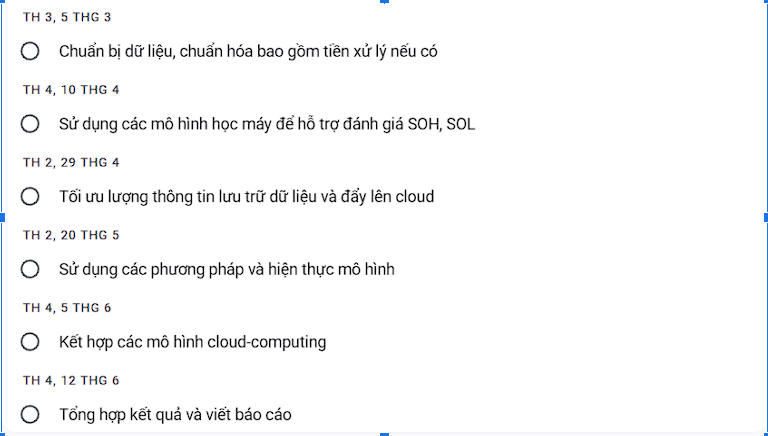
\includegraphics[width=5in]{plan.png}
\end{center}
\end{figure} 

\vspace{5cm}
\section{NỘI DUNG DỰ KIẾN CỦA LUẬN VĂN}

Nội dung báo cáo của luận văn dự kiến sẽ bao gồm các phần như sau:\\

\textbf{Chương 1: Giới thiệu}. Trong chương này sẽ trình bày một số vấn đề cơ bản của đề tài, nêu lên sự quan trọng của việc kiểm tra và giám sát thành phần trong xe điện trong lĩnh vực dữ liệu số hóa. Từ đó thấy được tầm quan trọng của đề tài để xác định rõ phạm vi và đối tượng nghiên cứu, hướng giải quyết của đề tài.
\\

\textbf{Chương 2: Các công trình nghiên cứu liên quan.} Trong chương này sẽ trình bày các công trình nghiên cứu liên quan. Tìm hiểu các phương pháp giải quyết vấn đề cũng như phạm vi, giới hạn của các nghiên cứu đó. Từ đó đánh giá tính khả thi của đề tài.\\

\textbf{Chương 3: Hiện thực và thử nghiệm mô hình. } Trong chương này sẽ trình bày chi tiết cách thức hiện thực của mô hình. Bao gồm các bước xây dựng và huấn luyện mô hình, sử dụng các mô hình và heuristic để giải quyết bài toán.\\

\textbf{Chương 4: Kết quả và đánh giá.} Trong chương này sẽ nêu ra các kết quả đạt được của mô hình, cũng như phương pháp đánh giá các kết quả đó.\\

\textbf{Chương 5: Kết luận.} Trong chương này sẽ tóm lại các ưu điểm và nhược điểm của mô hình và đưa ra các hướng nghiên cứu phát triển hệ thống trong tương lai.\\

\section{KẾT LUẬN}
Việc giám sát và quản lý pin đóng vai trò quan trọng trong đảm bảo hiệu suất, tuổi thọ và an toàn của hệ thống pin trên xe điện. Các công trình nghiên cứu liên quan đã tập trung vào các khía cạnh quan trọng như ước lượng trạng thái sạc và sức khỏe pin, chẩn đoán và tiên đoán lỗi, và quản lý thông minh của pin.\\

Để giám sát pin trên xe điện một cách hiệu quả, cần phải có hệ thống quản lý pin (BMS) thông minh và chính xác. BMS sẽ thu thập dữ liệu về trạng thái pin như trạng thái sạc, nhiệt độ, điện áp và dòng điện, sau đó phân tích và đưa ra các quyết định để bảo vệ pin và tối ưu hóa hiệu suất sử dụng năng lượng.\\

Công nghệ và phương pháp giám sát pin ngày càng phát triển, bao gồm sự kết hợp của cảm biến, hệ thống ghi dữ liệu, trí tuệ nhân tạo và học máy. Các phương pháp này giúp ước lượng trạng thái sạc và sức khỏe pin một cách chính xác, phát hiện và chẩn đoán lỗi một cách nhanh chóng, và dự đoán tuổi thọ còn lại của pin.\\

Thông qua việc nghiên cứu và áp dụng các công trình liên quan, có thể nâng cao hiệu suất và tuổi thọ của pin trên xe điện, giúp tăng khả năng di chuyển và đáp ứng nhu cầu của người sử dụng. Đồng thời, việc giám sát pin cũng đóng vai trò quan trọng trong việc đảm bảo an toàn và hạn chế các vấn đề liên quan đến pin như quá nhiệt, quá điện áp hoặc quá dòng điện.\\

Tổng quan, đề tài "Giám sát pin trên xe điện" là một lĩnh vực nghiên cứu quan trọng và đầy triển vọng, đóng góp vào sự phát triển của công nghệ pin và xe điện hiệu quả và bền vững.\\

\begin{thebibliography}{19}
    \bibitem
    [As87] Astrahan, M.M., Schkolnick, M., Whang, K.-Y. (1987)
    “Approximating the number of unique values of an attribute without
    sorting”, Journal Information Systems, Vol. 12 (1), pp. 11-15,
    Oxford, UK.
    
    \bibitem[Du03] Durand, M., Flajolet, P. (2003) “Loglog Counting of Large
    Cardinalities (Extended Abstract)”, In: G. Di Battista and U.
    Zwick (Eds.) - ESA 2003. Lecture Notes in Computer Science, Vol.
    2832, pp. 605-617, Springer, Heidelberg.
    
    \bibitem[Fl85] Flajolet, P., Martin, G.N. (1985) “Probabilistic Counting
    Algorithms for Data Base Applications”, Journal of Computer and
    System Sciences, Vol. 31 (2), pp. 182-209.
    
    \bibitem[Fl07] Flajolet, P., et al. (2007) “HyperLogLog: the analysis of a nearoptimal cardinality estimation algorithm”, Proceedings of the 2007
    International Conference on Analysis of Algorithms, Juan les Pins,
    France - June 17-22, 2007, pp. 127-146.
    
    \bibitem[He13] Heule, S., et al. (2013) “HyperLogLog in Practice: Algorithmic
    Engineering of a State of The Art Cardinality Estimation Algorithm”, Proceedings of the 16th International Conference on Extending
    Database Technology, Genoa, Italy —- March 18-22, 2013, pp. 683-
    692, ACM New York, NY.
    
    \bibitem[Sc07] Scheuermann, B., Mauve, M. (2007) “Near-optimal compression
    of probabilistic counting sketches for networking applications”,
    Proceedings of the 4th ACM SIGACT-SIGOPS International
    Workshop on Foundation of Mobile Computing (DIAL M-POMC),
    Portland, Oregon, USA. - August 16, 2007.
    
    \bibitem[Wh90] Whang, K.-Y., Vander-Zanden, B.T., Taylor H.M. (1990)
    “A Linear-Time Probabilistic Counting Algorithm for Database
    Applications”, Journal ACM Transactions on Database Systems,
    Vol. 15 (2), pp. 208-229.
\end{thebibliography}
\end{document}